\chapter{Desenvolvimento da Solução}
\label{chap:solucaocompleta}

\section{Metodologia}

Esse trabalho está dentro de um contexto específico na engenharia de software. Esse contexto se caracteriza num projeto de pesquisa e desenvolvimento no qual até a consolidação da solução pouco se sabia sobre sua natureza (por exemplo arquitetura e viabilidade), o andamento do desenvolvimento ocorreu de forma não-linear e complexa e houve um frequente diálogo entre disciplinas de diferentes domínios - transdiciplinaridade.

No que diz respeito ao desconhecimento da natureza da solução no início do projeto, houve várias questões teóricas de pesquisa que foram passíveis de experimentações e disscusões ao longo do processo de desenvolvimento. Tal fato ocasionou na caracterização da solução ao longo do projeto e sua definição total somente no final.

No que tange a não-linearidade, variou-se muito o desempenho na concretização de soluções. A taxa de produção intelectual comportou-se como não repetível ao longo do tempo. E a complexidade, de acordo com a teoria de Edgar Morin \cite{morin}, impactou o projeto de forma que a soma dos métodos e tecnologias gerasse resultados imprevisíveis.

O termo transdisciplinaridade é empregado para um patamar de relações entre disciplinas e domínios de conhecimento. Conceitua-se como tal um processo que transcende as disciplinas, que está entre, além e através das disciplinas \cite{criatividade}. Nesse trabalho foram investigados vários domínios de conhecimento como a engenharia, matemática, neurociências, psicologia, música e computação.

Dado o contexto e características do trabalho foi estabelicido um método de desenvolvimento empírico, iterativo e incremental. Na engenharia de software se destacam dois processos de controle de desenvolvimento: precesso definido e processo empírico. O processo definido é constiuído de um conjunto de sub-processos rigoros nos quais possuem entradas e saídas bem definidas e repetitivas \cite{rup}. Já o processo empírico é constituído de um conjunto de sub-processos imperfeitamente definidos nos quais as entradas e saídas são imprevisíveis e não repetíveis, características essas presentes no desenvolvimento desse trabalho.

A metodologia empírica de desenvolvimento de software se embasa em três fundamentos: precisa ser transparente, visto que o máximo de variáveis devem estar visíveis para os envolvidos no projeto; dado as variáveis expostas a metodologia precisa ser frequentemente inspecionada; feito as inspeções objetivo final é adaptar de acordo com as necessidades. Esses três fundamentos visam ajustar o processo de desenvolvimento para evitar variações de produção inaceitáveis e maximizar a mesma \cite{empirical}.

Para que os procedimentos da metodologia empírica possa ocorrer ela precisa ser de natureza iterativa e incremental. Iterativa e incremental pois terá ciclos curtos de desenvolvimento e a cada ciclo terá incrementos de código. No final de cada ciclo ter-se-à como resultado parâmetros de feedback para a melhoria contínua.

Outra análise do método empírico é o embasamento no ciclo de melhoria de processos e produtos $Plan$-$Do$-$Check$-$Act$ (PDCA) \cite{pdca}. Ele é constituído em 4 fases: $Plan$ - planejamento do desenvolvimento; $Do$ - executar o que foi planejado; $Check$ - avaliar o que foi feito; $Act$ - propor melhorias para os próximos ciclos.

% QUESTÕES
Com o intuito de atingir os objetivos, serão abordados questões, hipóteses e critérios relacionados às problemáticas abordadas. No que diz respeito as questões, segue a formulação das mesmas:
\begin{itemize}
	\item Se cada nota é uma frequência de vibração sonora, como analisar o sinal no ponto de vista de frequências? Dessa questão, surge a seguinte hipótese:
	\begin{itemize}
		\item A transformada de fourier pode construir o espectro de frequências do sinal. O critério para avaliar essa hipótese é:
			\begin{itemize}
				\item Vetor com os níveis de energia relacionados a cada frequência.		
			\end{itemize}
	\end{itemize}

	\item Como configurar essas informações para localizar as notas musicais?
	\begin{itemize}
		\item Dado que cada nota musical é um conjunto de frequências, realocar as energias frequenciais da transformada de fourier afim de que cada posição do vetor seje 1 unidedade de frequência (Hz) pode mapear a energia de cada nota. Os critérios para avaliar essa hipótese são:
			\begin{itemize}
				\item Vetor com os níveis de energia relacionados a cada frequência deve ter o tamanho de 22050 posições.
				\item Cada posição do vetor de energia relacionados a cada frequência possui valor de 1 Hz.		
			\end{itemize}
	\end{itemize}

	\item Como adicionar as próximas camadas da rede para determinação dos acordes?
	\begin{itemize}
		\item  Visto que associar as frequências as notas musicas é uma tarefa muito complexa para uma solução determinística, uma rede neural de aprendizado não supervisionado do tipo $Probabilistic Neural Network$ (PNN) pode classificar um conjunto de frequências em sua respectiva nota musical. O critério para avaliar essa hipótese é:
			\begin{itemize}
				\item Vetor com os níveis de energia relacionados a cada nota.		
			\end{itemize}
	\end{itemize}
	
	\item Como reconhecer acordes no tempo de tal forma a saber onde eles ocorrem?
	\begin{itemize}
		\item A transformada de fourier pode construir o espectro de frequências do sinal.
		O critério para avaliar essa hipótese é:
			\begin{itemize}
				\item Vetor com os níveis de energia relacionados a cada frequência.		
			\end{itemize}
	\end{itemize}
	\item Como ler o sinal todo e ter a visilibilidade em tempo e frequência?
	\begin{itemize}
		\item A transformada de fourier pode construir o espectro de frequências do sinal.
		O critério para avaliar essa hipótese é:
			\begin{itemize}
				\item Vetor com os níveis de energia relacionados a cada frequência.		
			\end{itemize}
	\end{itemize}
	\item Como ler o sinal todo e ter a visilibilidade em tempo e frequência?
	\begin{itemize}
		\item A transformada de fourier pode construir o espectro de frequências do sinal.
		O critério para avaliar essa hipótese é:
			\begin{itemize}
				\item Vetor com os níveis de energia relacionados a cada frequência.		
			\end{itemize}
	\end{itemize}
	\item Como extrair o tom da música?
	\begin{itemize}
		\item A transformada de fourier pode construir o espectro de frequências do sinal.
		O critério para avaliar essa hipótese é:
			\begin{itemize}
				\item Vetor com os níveis de energia relacionados a cada frequência.		
			\end{itemize}
	\end{itemize}
	\item Como trabalhar com a frequência de aparecimento das notas?
	\begin{itemize}
		\item A transformada de fourier pode construir o espectro de frequências do sinal.
		O critério para avaliar essa hipótese é:
			\begin{itemize}
				\item Vetor com os níveis de energia relacionados a cada frequência.		
			\end{itemize}
	\end{itemize}
	\item Em relação aos acordes transitórios, como corrigir?
	\begin{itemize}
		\item A transformada de fourier pode construir o espectro de frequências do sinal.
		O critério para avaliar essa hipótese é:
			\begin{itemize}
				\item Vetor com os níveis de energia relacionados a cada frequência.		
			\end{itemize}
	\end{itemize}
	\item Como extrair a nota mais grave (baixo) de cada período do tempo?
	\begin{itemize}
		\item A transformada de fourier pode construir o espectro de frequências do sinal.
		O critério para avaliar essa hipótese é:
			\begin{itemize}
				\item Vetor com os níveis de energia relacionados a cada frequência.		
			\end{itemize}
	\end{itemize}
	\item Como extrair a nota mais grave (baixo) de cada período do tempo e incluir os acordes aumentados e invertidos?
	\begin{itemize}
		\item A transformada de fourier pode construir o espectro de frequências do sinal.
		O critério para avaliar essa hipótese é:
			\begin{itemize}
				\item Vetor com os níveis de energia relacionados a cada frequência.		
			\end{itemize}
	\end{itemize}
\end{itemize}


\section{Técnicas Utilizadas para Desenvolvimento do Sistema-Solução}

Nesta secção será descrito o desenvolvimento da solução e as técnicas utilizadas. A explicação da solução se embasará no seguinte diagrama de fluxo de dados:

\begin{figure}[h]
	\centering
		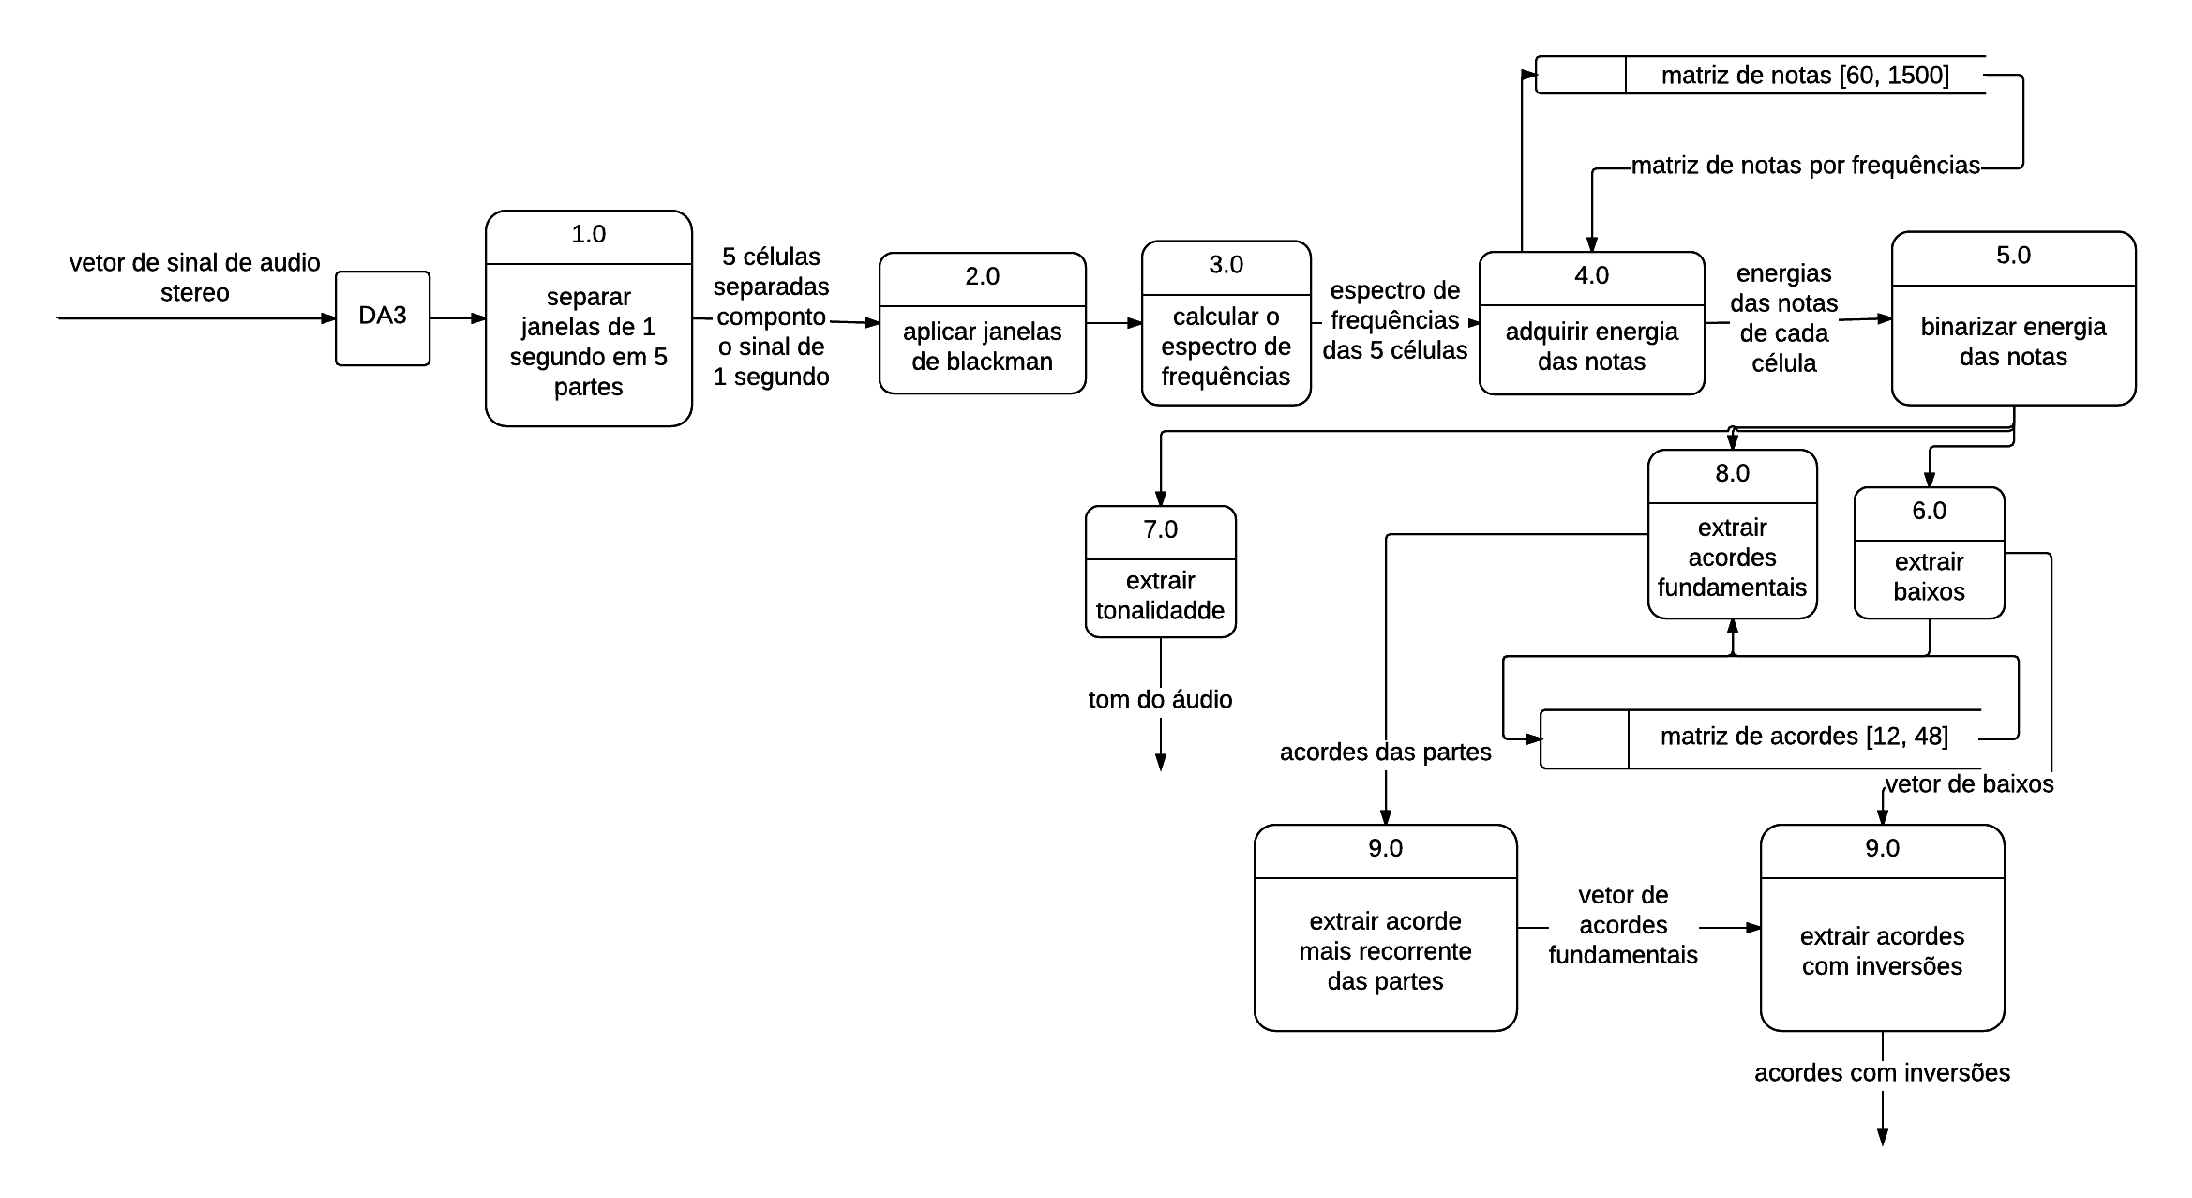
\includegraphics[keepaspectratio=true,scale=0.51]{figuras/dfd_2.eps}
	\caption{Diagrama de Fluxo de Dados}
\end{figure}

A solução começa com a chamada da função DA3. Ela recebe como parâmetro um vetor de audio $stereo$, ou seja, ela carrega uma matriz 2 por N, tal que N é o tamanho do sinal de áudio (número de amostras). Esse sinal de áudio é retornado através da função $wavread$($<$$caminho$ $do$ $arquivo$$>$$)$. O tipo de arquivo lido é do formato-padrão de áudio .wav. Esse formato de arquivo permite um armazenamento dos dados em blocos em modulação de pulsos PCM ($pulse$-$code$-$modulation$). O PCM armazena em arquivo de áudio não-comprimido (sem perdas), ou seja, o processo de amostragem e quantização representa exatamente o que foi descrito na parte de fundamentos teóricos desse trabalho (taxa de amostragem de 44.100 Hz e quantização de 16 bits). Ao final do fluxo há 2 saídas: os acordes ao longo do tempo e o tom do áudio.Nos próximos tópicos serão explicados os comportanmentos de cada uma das caixas de processamento do diagrama de fluxo de dados.

\subsection{Procedimento 1: Separar Janelas de 1 Segundo em 5 Partes}
\label{subsec:procedimento_1}

Após o sinal ser carregado num vetor de audio $stereo$, ele deverá ser transformado num do tipo mono. Sinal mono de áudio é aquele com somente um canal. Isso é necessário para que o processamento não fosse redundante. Não agregaria valor nesse caso processar um sinal de duplo canal sendo que a fonte emissora de ondas sonoras é comum para ambos. Após essa conversão o sinal é repartidos em 5 partes de tamanhos iguais a 1 segundo, porém deslocadas a 0.2 segundos de cada um. Esse processo é para a segmentar áudio no intuito de achar o acorde mais provável num intervalo de tempo de um segundo, fazendo com que acordes de transição ou ruidosos sejam suprimidos. A figura \ref{fig:procedimento_1} ilustra o processo descrito e o código do mesmo está presente na secção \ref{sec:codigo_procedimento_1} dos apêndices.

\begin{figure}[h] 
  \centering
    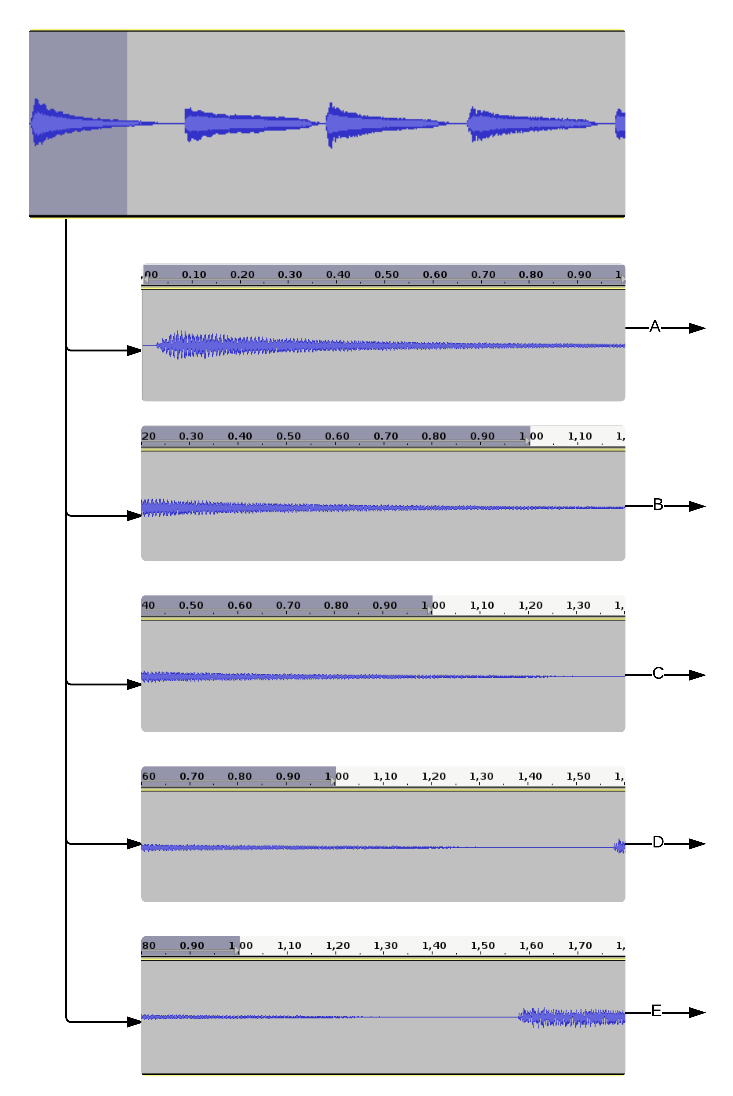
\includegraphics[keepaspectratio=true, scale=0.7]{figuras/procedimento_1}
    \caption{Ilustração do Procedimento 1}
    \label{fig:procedimento_1}
\end{figure}


Basicamente a variável de entrada dessa função é reescrita como uma matriz 1 por N, tal qual N é o número de amostras do sinal. No laço seguinte cria-se um conjunto de 5 células, cada uma comportando uma parte do sinal.

\subsection{Procedimento 2: Aplicar Janelas de Blackman}
\label{subsec:procedimento_2}

Dado que o contexto da solução se deu por $Short$-$Time$-$Fourier$-$Transform$, é preciso minimizar as distorções oriundas dos janelamentos. Para tal foi proposto a multiplicação de cada parte das janelas ao longo do tempo por uma janela de blackman, uma do tipo gaussiana. A figura \ref{fig:procedimento_2} ilustra o processo descrito e o código do mesmo está presente na secção \ref{sec:codigo_procedimento_2} dos apêndices.

\begin{figure}[h] 
  \centering
    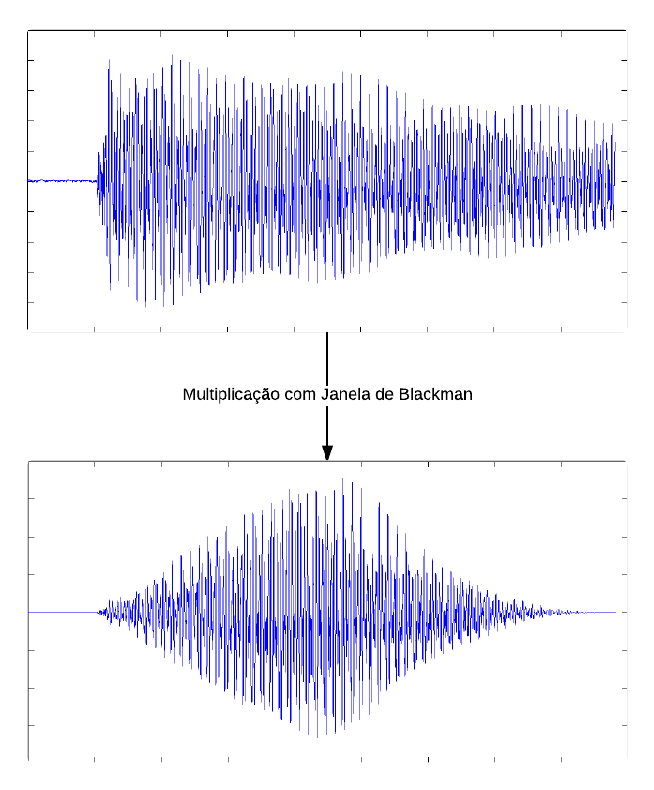
\includegraphics[keepaspectratio=true, scale=0.7]{figuras/procedimento_2}
    \caption{Ilustração do Procedimento 2}
    \label{fig:procedimento_2}
\end{figure}

\subsection{Procedimento 3: Calcular o Espectro de Frequências}
\label{subsec:procedimento_3}

O passo seguinte é adquirir os espectros de frequências oriundos do cálculo da transformada discreta de fourier. O cálculo será feito para cada uma das 5 partes de janelas. A figura \ref{fig:procedimento_3} ilustra o processo descrito e o código do mesmo está presente na secção \ref{sec:codigo_procedimento_3} dos apêndices.

\begin{figure}[h] 
  \centering
    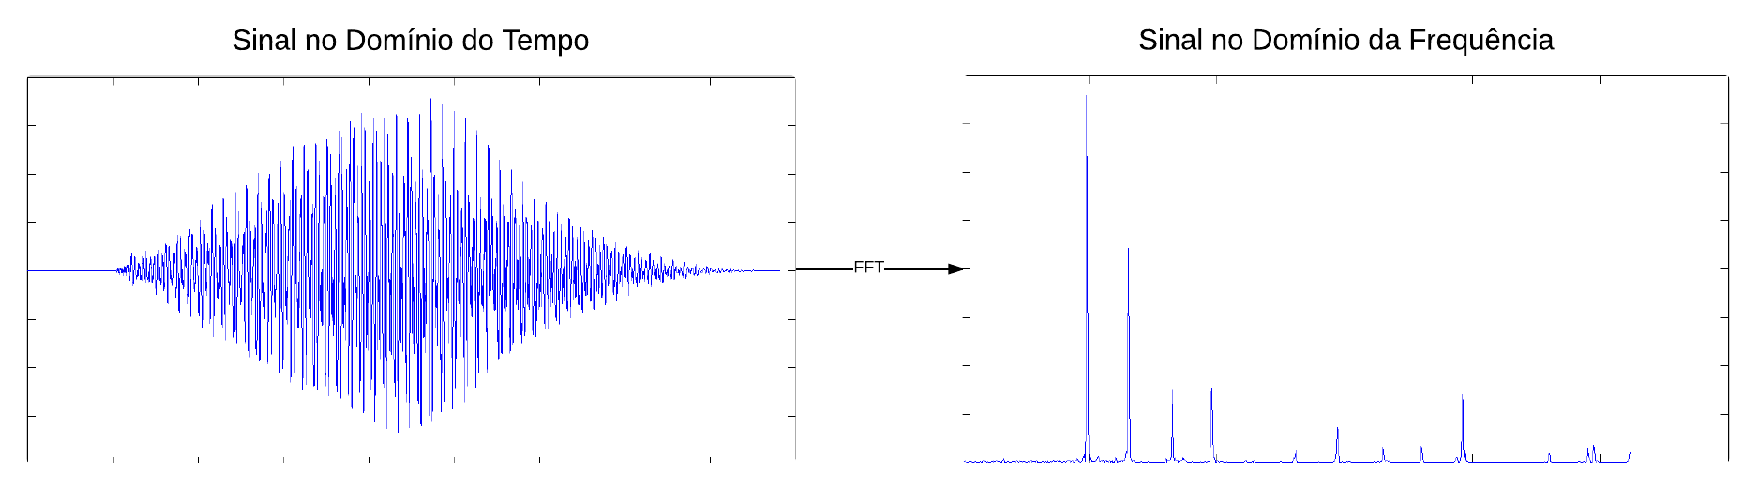
\includegraphics[keepaspectratio=true, scale=0.5]{figuras/procedimento_3}
    \caption{Ilustração do Procedimento 3}
    \label{fig:procedimento_3}
\end{figure}

Primeiramente é alocado uma variável para comportar os 5 espectros de frequência, um para cada parte da janela. Depois os sinais passam por uma transformação de subamostragem na qual são eliminadas informações de altas frequências a partir de 1500 Hz. É feito o cálculo do módulo da transformada de frourier e esse mesmo vetor passar por uma reorganização de $slots$ de tal forma que cada $slot$ comporta-se 1 unidade de Hz.

\subsection{Procedimento 4: Adquirir Energias das Notas}
\label{subsec:procedimento_4}

Nesse procedimento cada espectro de frequência é correlacionado com conjunto de notas musicais dado um conjunto de frequências que nelas estão presentes. A figura \ref{fig:procedimento_4} ilustra o processo descrito e o código do mesmo está presente na secção \ref{sec:codigo_procedimento_4} dos apêndices.

\begin{figure}[h] 
  \centering
    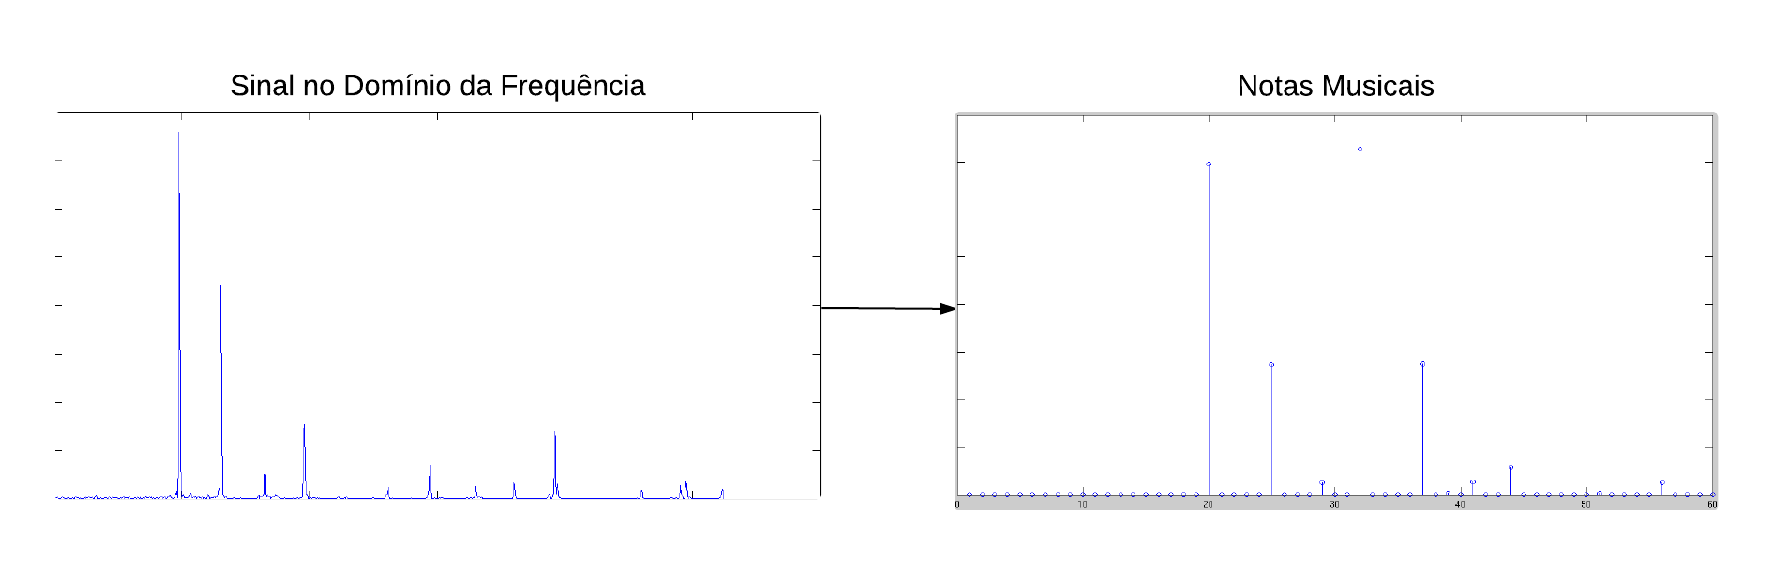
\includegraphics[keepaspectratio=true, scale=0.55]{figuras/procedimento_4}
    \caption{Ilustração do Procedimento 4}
    \label{fig:procedimento_4}
\end{figure}

A primeira atividade é carregar a base de dados de notas musicais originando o retorno de um matriz 60 notas por 1500 frequências. Então cada conjunto de notas relacionados às partes de janela serão correlacionados a partir de uma operação de multiplicação e, por fim, é feita a soma dos quadrados dos termos. Ao final uma matriz de notas por tempo é construída para cada uma das 5 partes.

\subsection{Procedimento 5: Binarizar Energia das Notas}
\label{subsec:procedimento_5}

Esse passo compreende o processo de limiarização das energias das notas em 0's ou 1's de tal forma que se possa detectas as notas tocadas (1) ou não (0). Ao final desse processo espera-se conjuntos de energias de notas musicais em somente dois valores - 1 ou 0. A figura \ref{fig:procedimento_5} ilustra o processo descrito e o código do mesmo está presente na secção \ref{sec:codigo_procedimento_5} dos apêndices.

\begin{figure}[h] 
  \centering
    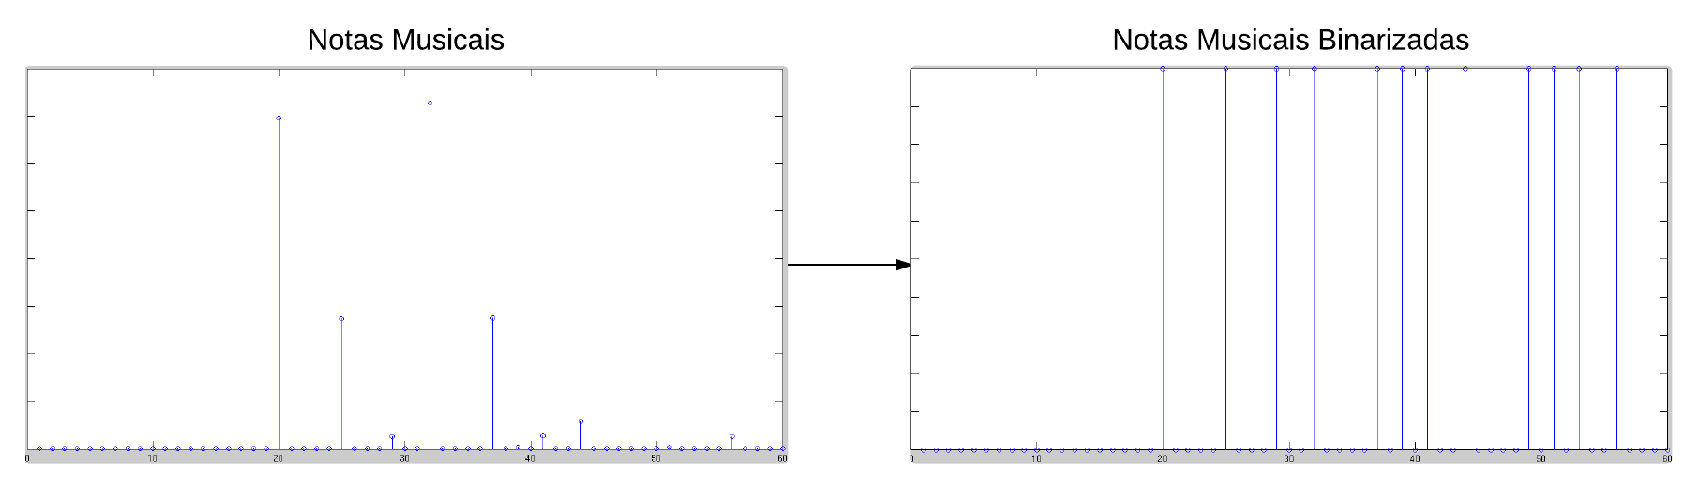
\includegraphics[keepaspectratio=true, scale=0.55]{figuras/procedimento_5}
    \caption{Ilustração do Procedimento 5}
    \label{fig:procedimento_5}
\end{figure}

No começo do procedimento é destacado um laço para cada uma das partes das janelas. No meio do procedimento destaca-se com operação de realocação do valor 0 para valores de energia menores que 180\% do valor máximo do conjunto de notas e 1 se for caso ao contrário. Por fim cada conjunto de notas são realocados em células.

\subsection{Procedimento 6: Extrair Baixos}
\label{subsec:procedimento_6}

Com o intuito de determinar acordes com inversões e discernir os que são de natureza aumentada, acoplou-se no sistema um componente desenvolvido para a extração das notas mais graves numa dada janela de tempo. A figura \ref{fig:procedimento_6} ilustra o processo descrito e o código do mesmo está presente na secção \ref{sec:codigo_procedimento_6} dos apêndices.

\begin{figure}[h] 
  \centering
    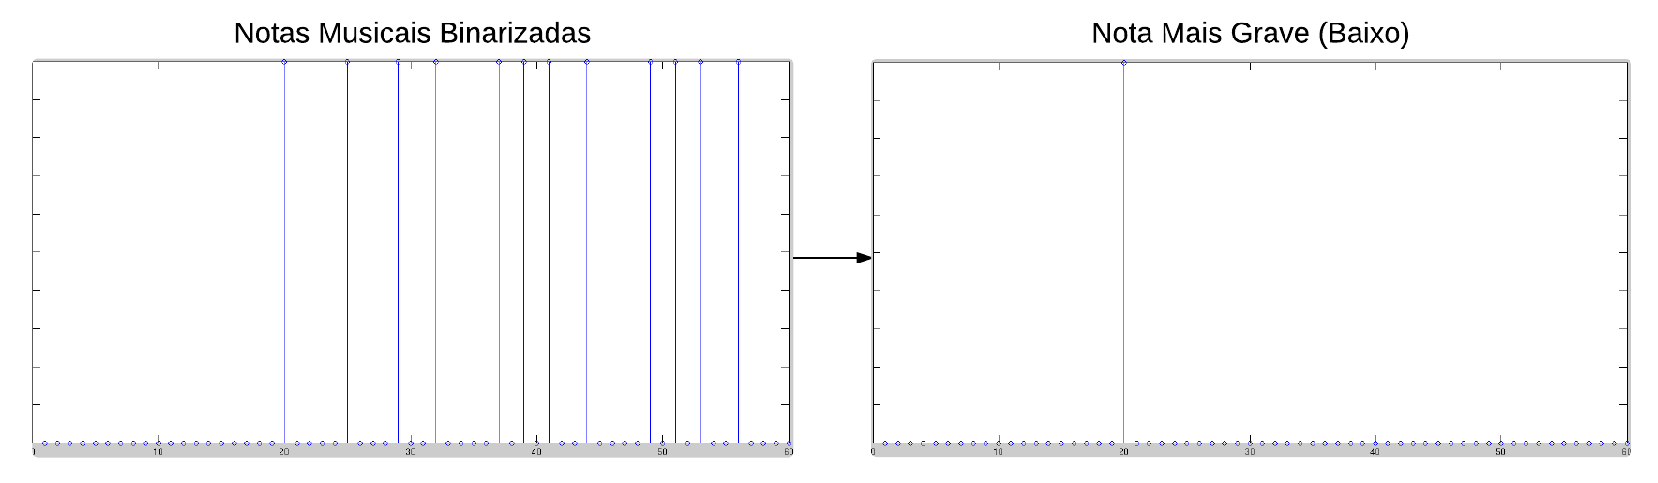
\includegraphics[keepaspectratio=true, scale=0.55]{figuras/procedimento_6}
    \caption{Ilustração do Procedimento 6}
    \label{fig:procedimento_6}
\end{figure}

No procedimento verificamos que os primeiros passos são de atribuição de variáveis em relação as partes das janelas. Depois cada uma dessas partes serão analisadas quanto as notas mais recorrentes com a função \textbf{mode}. Dado essa análise os baixos são extraidos com a primeira ocorrência de 1, dado que as notas estão binarizadas.

\subsection{Procedimento 7: Extrair Tonalidade}
\label{subsec:procedimento_7}

A extração de tonalidade é um módulo do sistema que possui como entrada o conjunto de notas binarizadas das partes de janela. A saída é o tom da música tocado baseando-se em acordes fundamentais maiores e menores. A figura \ref{fig:procedimento_7} ilustra o processo descrito e o código do mesmo está presente na secção \ref{sec:codigo_procedimento_7} dos apêndices. 

\begin{figure}[h] 
  \centering
    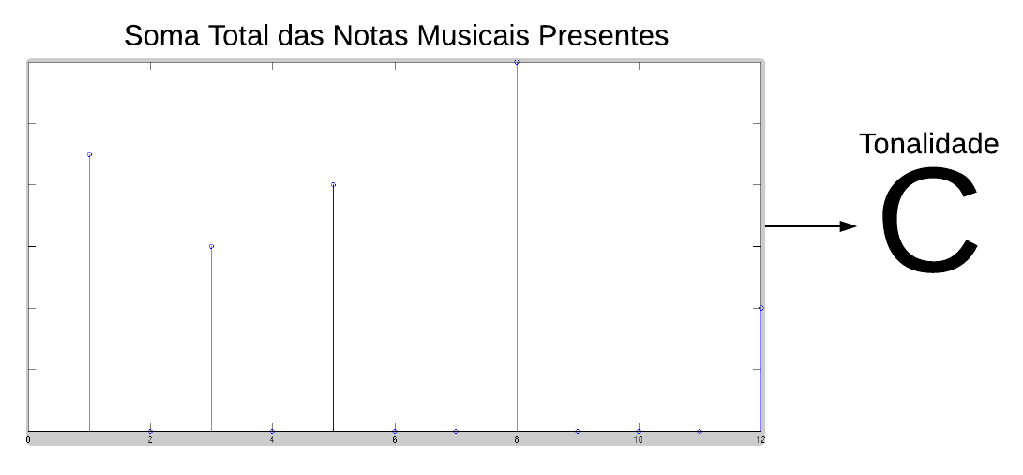
\includegraphics[keepaspectratio=true, scale=0.55]{figuras/procedimento_7}
    \caption{Ilustração do Procedimento 7}
    \label{fig:procedimento_7}
\end{figure}

No início desse processo há declaração nominal dos acordes em tipo string. Após o conjunto de notas em relação são somadas, cada uma na sua respectiva frequência, para gerar um vetor que totaliza a soma das frequências tocadas ao longo de todo áudio. O procedimento seguinte, focando extrair um acorde desse vetor de notas ao longo de todo áudio, é utilizado uma correlação do mesmo com uma base dados carregada de notas pelos respectivos acordes. Ao final cada acorde da base de dados terá sua energia correspondente e, ao extrair o máximo das energias, é adquirido o acorde tom da música.

\subsection{Procedimento 8: Extrair Acordes Fundamentais}
\label{subsec:procedimento_8}

A extração de acordes fundamentais é um módulo do sistema que possui como entrada o conjunto de notas binarizadas das partes de janela. A saída é um conjunto de acordes fundamentais ao longo do tempo. A figura \ref{fig:procedimento_8} ilustra o processo descrito e o código do mesmo está presente na secção \ref{sec:codigo_procedimento_8} dos apêndices.

\begin{figure}[h] 
  \centering
    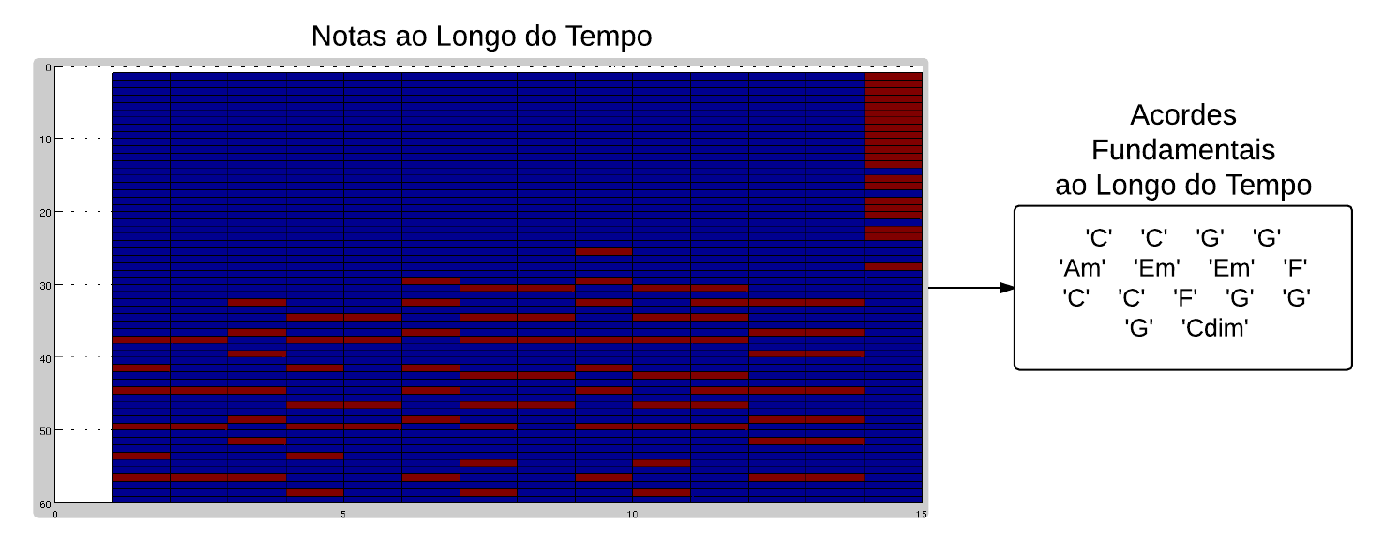
\includegraphics[keepaspectratio=true, scale=0.55]{figuras/procedimento_8}
    \caption{Ilustração do Procedimento 8}
    \label{fig:procedimento_8}
\end{figure}


No início desse processo há o carregamento da base de dados de acordes em relação as notas musicais. Após o conjunto de notas são somadas em relação às respectivas oitavas gerando vetor de somente 12 posições. Esse mesmo vetor é submetido então a um processo de correlação aos acordes derivados da base de dados. Ao final cada acorde da base de dados terá sua energia correspondente e, ao extrair o máximo das energias, é adquirido os acordes fundamentais ao longo do tempo.

\subsection{Procedimento 9: Extrair Acorde Recorrente das Partes}
\label{subsec:procedimento_9}

A extração de acorde recorrente é um módulo do sistema que possui como entrada o conjunto de acordes das partes de janela. A saída são acordes fundamentais ao longo do tempo com eliminação das 5 partes. A figura \ref{fig:procedimento_9} ilustra o processo descrito e o código do mesmo está presente na secção \ref{sec:codigo_procedimento_9} dos apêndices.

\begin{figure}[h] 
  \centering
    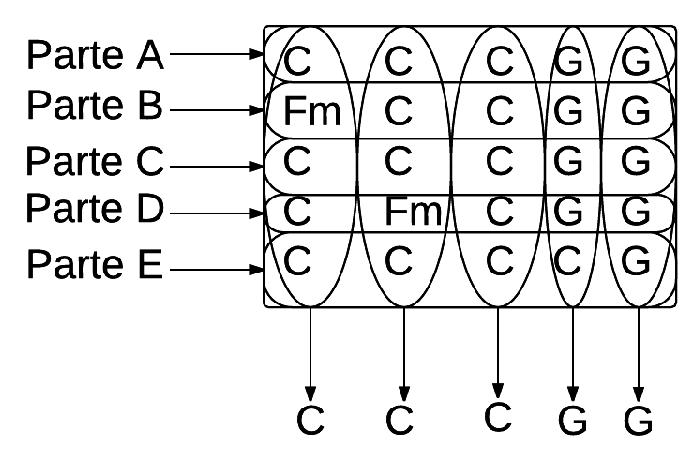
\includegraphics[keepaspectratio=true, scale=0.55]{figuras/procedimento_9}
    \caption{Ilustração do Procedimento 9}
    \label{fig:procedimento_9}
\end{figure}

No início desse processo há a atribuição de variáveis a cada uma das 5 partes. Após o conjunto das partes em acordes é submetido a função \textbf{mode} para extrair o acorde mais recorrente dentro de uma dada faixa de tempo do áudio.


\subsection{Procedimento 10: Extrair Acordes com Inversões}
\label{subsec:procedimento_10}

Da última etapa do sistema, a extração de acordes com inversões tem como finalidade formar acordes invertidos a partir da entrada dos acordes fundamentais e os baixos. A figura \ref{fig:procedimento_10} ilustra o processo descrito e o código do mesmo está presente na secção \ref{sec:codigo_procedimento_10} dos apêndices.

\begin{figure}[h] 
  \centering
    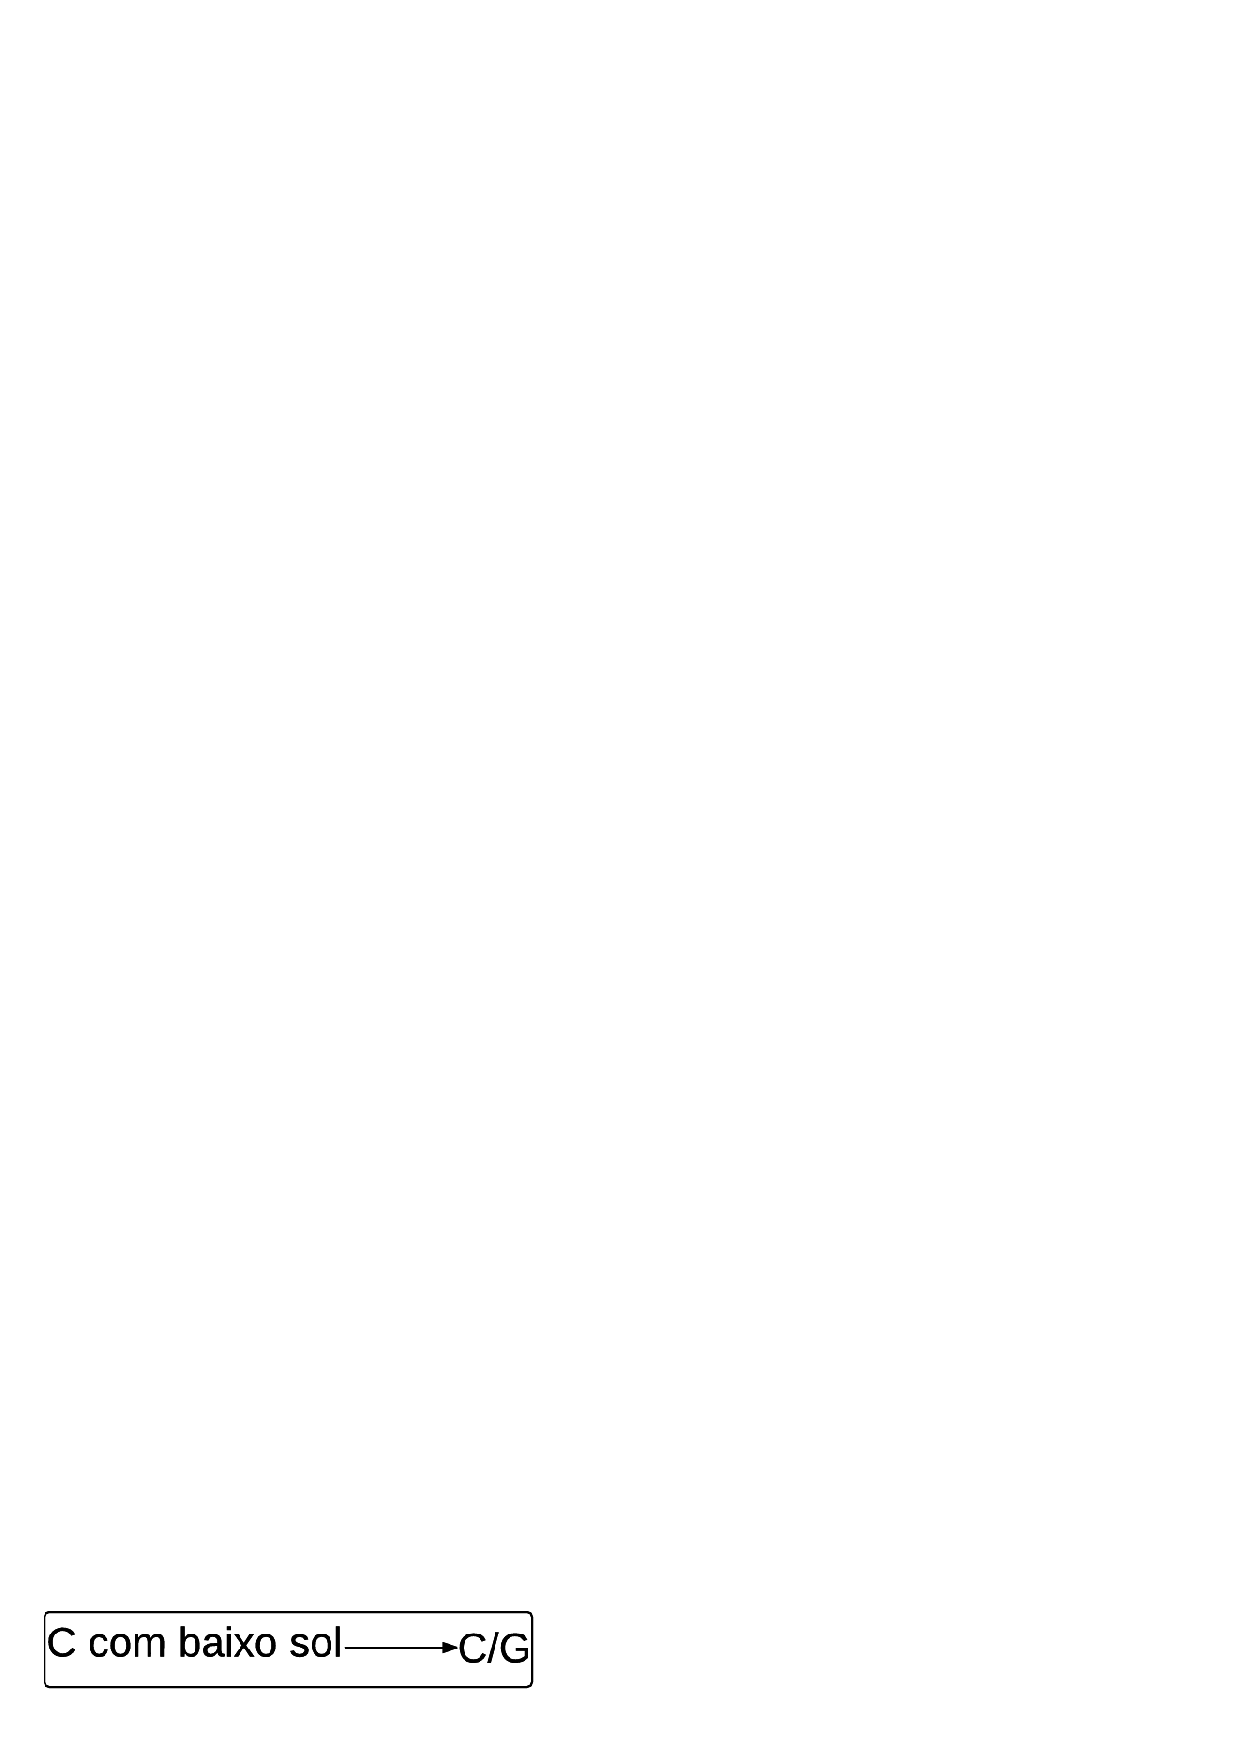
\includegraphics[keepaspectratio=true, scale=0.55]{figuras/procedimento_10}
    \caption{Ilustração do Procedimento 10}
    \label{fig:procedimento_10}
\end{figure}

No início desse processo há o carregamento de um vetor de acordes, cada um com uma nomeclatura de acorde. Após é construído pares de acordes e baixos para mapear os acordes tocados dentro do vetor de acordes nominais. Ao final do processo as células de acordes e baixos identificados são referenciados dentro do vetor de acordes nominais com inversões, através das células de pares de acordes e baixos.



\section {Ciclos de Desenvolvimento}
 
Nesta presente parte do trabalho será descrito os ciclos de desenvolvimento para a construção do sistema-solução. Os detalhes e o código completo podem ser encontrados no repositório $github$ \footnote{https://github.com/josepedro/TCC}.

\subsection{Estrutura do Ciclo}

\begin{figure}[h] 
  \centering
    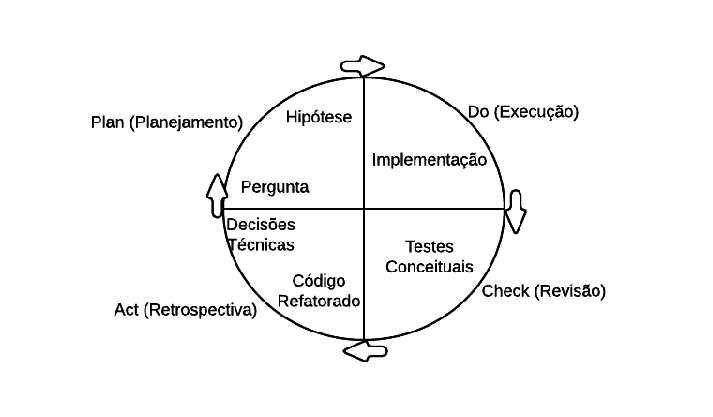
\includegraphics[keepaspectratio=true, scale=0.85]{figuras/ciclo_desenvolvimento}
    \caption{Modelo de Ciclo Adaptado}
\end{figure}

Fases do ciclo de desenvolvimento:
\begin{itemize}
\item \textbf{Pergunta:} No início de cada ciclo é feito uma pergunta a ser respondida que se adere aos objetivos do trabalho.
\item \textbf{Hipótese:} A partir dessa pergunta é feita hipóteses que possam responder;
\item \textbf{Implementação:} As hipóteses são pensadas, construidas e implementadas num script;
\item \textbf{Testes Conceituais:} Cada hipótese implementada é testada conforme a teoria usada;
\item \textbf{Retrospectiva:} Dado os resultados dos testes conceituais e código refatorado, é feitto uma avaliação do que foi produzido e decisões técnicas são tomadas.
\end{itemize}
  
\subsection{Ciclo 1}
\label{subsec:ciclo_1}

\begin{itemize}
\item \textbf{Pergunta:} Para saber da harmonia da música é preciso saber as notas dela. Se cada nota é uma frequência de vibração sonora, como analisar o sinal no ponto de vista de frequências? É possível?
\item \textbf{Hipótese:} A Transformada de Fourier pode construir o espectro de frequências do sinal.
\item \textbf{Implementação:} 
\begin{lstlisting}
som = som(1:length(som));
som = som/max(som);
t = fft(som);
SINAL=sqrt(t.*conj(t));
SINAL=SINAL/max(SINAL);
\end{lstlisting}
\item \textbf{Testes Conceituais:} Testes foram feitos para ver se os picos de frequência correspondem ao sinal de entrada. O resultado foi positivo e os picos representam a energia das frequências;
\item \textbf{Retrospectiva:} A Transformada de Fourier, em específico a $Fast Fourier Transform$, realmente produz resultados satisfatórios em determinar o espectro de energia da frequências. Mas as informações não estão configuradas para localizar as notas musicais.
\end{itemize}

\subsection{Ciclo 2}
\label{subsec:ciclo_2}
\begin{itemize}
\item \textbf{Pergunta:} Como configurar essas informações para localizar as notas musicais?
\item \textbf{Hipótese:} Dado que cada nota musical é um conjunto de frequências, realocar as energias frequenciais da transformada de fourier afim de que cada posição do vetor seje 1 unidedade de frequência (Hz) pode mapear a energia de cada nota.
\item \textbf{Implementação:} 
\begin{lstlisting}
fs = 44100;
f = (0:length(som)-1)*fs/length(som);
freq = f(1:round(length(f)/2));
SOM = abs(fft(som));
SOM = SOM/max(SOM);
SOM = SOM(1:round(length(f)/2));
l = 1;
j = 0;
i = 1;
SOMA = 0; 
while (i<length(freq))
    if (round(freq(i)) == round(freq(i+1)))
        SOMA = SOM(i+1) + SOMA;
        j = j + 1;
    else
        respfreq(l) = SOMA/(j+1);
        j = 0;
        SOMA = SOM(i+1);
        l = l+1;
    end
    i = i+1;
end
l = 0; j = 0; i = 0;
\end{lstlisting}
\item \textbf{Testes Conceituais:} De fato as notas musicais foram localizadas com mais facilidade em determinados grupos de frequências. Tal ordenamento de frequências resultou num vetor de 22050 posições, independentemente do tamanho da amostra.
\item \textbf{Retrospectiva:} A estratégia de realocar as energias decimais das frequências numa unidade de frequência se adere corretamente ao objetivo de encontrar as notas musicais. Entretanto as frequências não estão associadas as notas musicais.
\end{itemize}

\subsection{Ciclo 3}
\label{subsec:ciclo_3}
\begin{itemize}
\item \textbf{Pergunta:} Dado um conjunto de frequências, como associar essas as notas musicais?
\item \textbf{Hipótese:} Visto que associar as frequências as notas musicas é uma tarefa muito complexa para uma solução determinística, uma rede neural de aprendizado não supervisionado do tipo $Probabilistic Neural Network$ (PNN) pode classificar um conjunto de frequências em sua respectiva nota musical.
\item \textbf{Implementação:} 
\begin{lstlisting}
%BASE DE DADOS DE NOTAS MUSICAIS DA REDE NEURAL
%NOTAS
notas(12,22050) = 0; %matriz das notas
%Do grave
notas(1,61) = 0.1;
notas(1,62) = 0.2;
notas(1,63) = 0.4;
notas(1,64) = 0.6;
notas(1,65) = 0.8;
notas(1,66) = 1;
notas(1,67) = 0.8;
notas(1,68) = 0.6;
notas(1,69) = 0.4;
notas(1,70) = 0.2;
notas(1,71) = 0.1;
.
.
.
i = 1; %contador para andar ao longo do vetor
b = 0.15; %sensibilidade da rede
while (i <= 12)
     %S1(i) = exp(-(norm(rfeq - notas(i,:))*b));
     %correlacao = corrcoef(rfeq,notas(i,:));
     %S1(i) = correlacao(1,2);    
     S1(i) = sum(abs(rfeq.* notas(i,:)));

    i = i + 1;
end

\end{lstlisting}
\item \textbf{Testes Conceituais:} Foram testadas 3 funções de transferência do neurônio. A primeira função de transferência - a exponencial da subtração dos valores - não foi muito eficaz pois para notas adjacentes as mesmas eram confundidas pela rede. Esse fato se dá pelo retorno de baixa magnitude da subtração de valores. A segunda função de transferência - a correlação dos valores - foi bastante eficaz para caracterizar notas. Porém a operação de subtração da média faz com que a energia final seja baixa, além de requisitar mais operações. A terceira função de transferência - a multiplicação dos valores - foi bastante eficaz para caracterizar notas e é rápida pois é uma forma simples da segunda função de transferência.
\item \textbf{Retrospectiva:} A rede neural PNN foi bastante eficaz em classificar as frequências em termos de notas musicais. Porém as notas musicais não estão associadas a acordes musicais.
\end{itemize}

\subsection{Ciclo 4}
\label{subsec:ciclo_4}
\begin{itemize}
\item \textbf{Pergunta:} Como adicionar as próximas camadas da rede para determinação dos acordes?
\item \textbf{Hipótese:} Para poder mapear as notas é preciso adicionar mais 2 camadas. Uma camada para classificação de acordes, dado um conjunto de notas musicais e a outra para classificação de um acorde dado os conjuntos possíveis de acordes.
\item \textbf{Implementação:} 
\begin{lstlisting}
% BASE DE DADOS PARA ACORDES

%--------------------------
BD(12,48) = 0;
%--------------------------

afin1 = 0; afin2 = 0;

%C
%CM
BD(12,1) = afin1;
BD(1,1) = 1; %baixo
BD(2,1) = afin2;
BD(4,1) = afin1;
BD(5,1) = 1; %terca
BD(6,1) = afin2;
BD(7,1) = afin1;
BD(8,1) = 1; %quinta
BD(9,1) = afin2;

.
.
.
%(430 LINHAS DE ACORDES)

%RADIAL BASIS LAYER para BD notas

while (i <= 48)
    S2(i) = sum(abs(S1.* BD(i,:)));
    i = i + 1;
end

\end{lstlisting}
\item \textbf{Testes Conceituais:} Foram testadas todas as possibilidades de acordes e os que não foram evetivamente reconhecido foram as inversões e os acordes aumentados.
\item \textbf{Retrospectiva:} De certo o acerto não foi total pois falta implementar uma camada que reconheça inversões.
\end{itemize}

\subsection{Ciclo 5}
\label{subsec:ciclo_5}
\begin{itemize}
\item \textbf{Pergunta:} Como reconhecer acordes no tempo de tal forma a saber onde eles ocorrem?
\item \textbf{Hipótese:} Uma solução de reconhecimento de energias ao longo do tempo pode ser eficaz para a determinação do rítmo. Em tese é calcular a energia do sinal e aplicar um filtro passa-baixas para identificação dos picos de energia.
\item \textbf{Implementação:} 
\begin{lstlisting}
    % opening the file
    file = open(file_path);
    file.data = file.data(1 : file.fs*4);
    bpm_music = abs(file.data);
    %filtering the pulses of minor energy
    signal_filtered = filter_signal(bpm_music);
    % Building array with means movies
    %signal_pulses = decrease_resolution(signal_filtered, file.fs, 1000);
    signal_pulses = downsample(signal_filtered, 22050);
    % Beginnnig the correlation
    array_correlation = correlate_moments(signal_pulses);

\end{lstlisting}
\item \textbf{Testes Conceituais:} Para um caso específico a solução funcionou, porém os outros casos ela não se aderiu.    
\item \textbf{Retrospectiva:} De certo modo detectar onde acorde ocorre no sinal não agrega valor para o escopo desse trabalho pois os níveis de energia são muito variáveis e não há um padrão como para a detecção.
\end{itemize} 

\subsection{Ciclo 6}
\label{subsec:ciclo_6}
\begin{itemize}
\item \textbf{Pergunta:} Como ler o sinal todo e ter a visilibilidade dele em tempo e frequência?
\item \textbf{Hipótese:} Para se ter uma resolução completa do sinal em tempo em frequência é preciso de ter uma transformada que agregue esses dois aspectos. Poder testar isso com a transformada wavelets.   
\item \textbf{Implementação:} 
\begin{lstlisting}
function [signal, imin, imax, iterations, energy] = ...
tree_iterator(signal, mini, maxi, imin, imax, iterations, energy)

if iterations == 0
	if mini >= 1 && maxi <= 22050
	  [signal, imin, imax, iterations, energy] = ...
	  tree_iterator(signal, mini, maxi, 1, 22050, 1, 0);
	else
	  imin = 1;
	  imax = 22050;
	  return;
end
elseif iterations > 0
	imean = (imax - imin)/2 + imin;
	%Low
	if mini >= imin && maxi <= imean
	  [h0, h1] = wfilters('db45');
	  [signal, y1] = decomposition_1level_qmf(h0, h1, signal);
	  energy = sum(abs(signal)) + energy;
	  iterations = iterations + 1;
	  imax = imean;
	  [signal, imin, imax, iterations, energy] = ...
	  tree_iterator(signal, mini, maxi, imin, ...
	  imax, iterations, energy);
	%High 
	elseif mini >= imean && maxi <= imax
	  [h0, h1] = wfilters('db45');
	  [y0, signal] = decomposition_1level_qmf(h0, h1, signal);
	  energy = sum(abs(signal)) + energy;
	  iterations = iterations + 1;
	  imin = imean;
	  [signal, imin, imax, iterations, energy] = ...
	  tree_iterator(signal, mini, maxi, ...
	  imin, imax, iterations, energy);
	else
	  return;
	end
end

\end{lstlisting}
\item \textbf{Testes Conceituais:} A solução falhou num teste muito simples. Ao submeter um sinal puro numa frequencia determinada e constante o banco de filtros wavelets distorcia o sinal, deslocando a fase do sinal para frequencias adjacentes da original.
\item \textbf{Retrospectiva:} Dado a barreira técnica de deslocamento de fase do sinal, ainda não foi encontrado uma solução de resolução tempo-frequência.
\end{itemize}

\subsection{Ciclo 7}
\label{subsec:ciclo_7}
\begin{itemize}
\item \textbf{Pergunta:} Como ler o sinal todo e ter a visilibilidade dele em tempo e frequência?
\item \textbf{Hipótese:} Para se ter uma resolução completa do sinal em tempo em frequência é preciso de ter uma transformada que agregue esses dois aspectos. Poder testar isso com a $Short Fourier Transform$ (Transformada de Fourier Janelada).   
\item \textbf{Implementação:} 
\begin{lstlisting}
function [notes_time, chords_time, chord_pitch] = DA3(signal, fs)

load_notes;
load_chords;
.
.
.
% begin to analyse music
time_seconds_total = fix((length(signal)/fs));
notes_time(time_seconds_total, 60) = 0;
chords_time = {};
for time = 1:time_seconds_total
    signal_time = signal(1+((time-1)*fs):time*fs);
    window = blackman(length(signal_time));
    signal_time = window'.*signal_time;
    signal_time = downsample(signal_time, 21);
    fs_time = fs/21;
    module_fft = abs(fft(signal_time));
    respfreq(1:fs_time) = 0;
    window_mean = length(signal_time)/fs_time;
    for frequency = 1:fs_time
        respfreq(frequency) = sum(module_fft( ...
        1+((frequency-1)*window_mean):frequency* ...
        window_mean))/window_mean;
    end
    respfreq = respfreq(1:fix(length(respfreq)/2));
    for note = 1:60
        notes_time(time, note) = sum(respfreq.* ...
        notes(note,:));    
    end
    energy_chords(1:48) = 0;
    for chord = 1:48
        energy_chords(chord) = sum(notes_time(time, :) ...
        .*chords(chord,:));
    end
    chords_time{time} = dictionary_chords{ ...
    find(energy_chords==max(energy_chords))};
end
notes_energy_total = notes_time(1,:);
for time = 2:time_seconds_total
    notes_energy_total = notes_energy_total + notes_time(time,:);
end
energy_chords(1:48) = 0;
for chord = 1:48
    energy_chords(chord) = sum(notes_energy_total.*chords(chord,:));
end
chord_pitch = dictionary_chords{find(energy_chords== ...
max(energy_chords))};
\end{lstlisting}
\item \textbf{Testes Conceituais:} A solução da transformada de fourier janelada foi testada com acordes de violão e piano ao longo do tempo e o resultado foi satisfatório exceto para acordes de transição.
\item \textbf{Retrospectiva:} A solução da transformada de fourier janelada se encaixou bem no conjunto.  
\end{itemize}

\subsection{Ciclo 8}
\label{subsec:ciclo_8}
\begin{itemize}
\item \textbf{Pergunta:} Como extrair o tom da música?
\item \textbf{Hipótese:} Para extrair o tom da música é preciso somar a energia das notas totais ao longo da música.
\item \textbf{Implementação:} 
\begin{lstlisting}
function [chord_pitch, chord_pitch_number] = ...
get_chord_pitch(notes_time, time_seconds_total, chords)
  
  dictionary_chords = ...
.
.
.
  notes_energy_total(60) = 0;
  for note = 1:60
    notes_energy_total(note) = sum([notes_time(:,note)]);
  end

  % discover tone music
  notes_energy_tone(12) = 0;
  for note = 1:12
    notes_energy_tone(note) = notes_energy_total(note) ...
     + notes_energy_total(note + 12) ...
      + notes_energy_total(note + 2*12) + ...
      notes_energy_total(note + 3*12) ...
        + notes_energy_total(note + 4*12);
  end

  % find chord tone
  load_chords_tone;
  chords_tone(48) = 0;
  for chord = 1:48
    chords_tone(chord) = sum((notes_energy_tone.* ...
    chords_tone_mask(:, chord)'.^2));
  end

  chord_pitch_number = find(chords_tone==max(chords_tone));
  chord_pitch = dictionary_chords{chord_pitch_number};
\end{lstlisting}
\item \textbf{Testes Conceituais:} A solução foi testada com sequencia de acordes do violão e as vezes o tom não é o certo.
\item \textbf{Retrospectiva:} A quantidade de energia está atrapalhando a extração do tom. O tom é definido como a frequência de aparecimento das notas ao longo da música.
\end{itemize}

\subsection{Ciclo 9}
\label{subsec:ciclo_9}
\begin{itemize}
\item \textbf{Pergunta:} Como trabalhar com a frequencia de aparecimento das notas?
\item \textbf{Hipótese:} Se binarizar com 1 e 0 o mapa de notas no tempo a soma das notas será unitária, equivalente a frequência.
\item \textbf{Implementação:} 
\begin{lstlisting}
% binarize set of notes
    for set = 1:5
        notes_time = set_of_notes_time{set};
        
        for time = 1:time_seconds_total
            for note = 1:60
                if notes_time(time, note) < max(max(notes_time))/180
                    notes_time(time, note) = 0;
                else
                    notes_time(time, note) = 1;
                end
            end
        end

        set_of_notes_time{set} = notes_time;
    end
\end{lstlisting}
\item \textbf{Testes Conceituais:} A solução foi testada e verificada com picos somente de 1 e vales somente de 0. 
\item \textbf{Retrospectiva:} Com essa binarização o tom da música foi efetivamente corrigido.
\end{itemize}

\subsection{Ciclo 10}
\label{subsec:ciclo_10}
\begin{itemize}
\item \textbf{Pergunta:} Em relação aos acordes transitórios, como corrigir?
\item \textbf{Hipótese:} Se ao deslocar a janela de tamanho de 1 segundo em passos de 0.2 segundos e calcular o espectro de frequência de cada passo pode-se fazer a média do acorde de cada tempo e poder cancelar os acordes transitórios.
\item \textbf{Implementação:}
\begin{lstlisting}
function set_of_windows_signals = ...
build_window_short_fft(signal, time, fs)
  signal = [signal(:)];

    % part A
    time_start_A = round(1+((time-1)*fs));
    time_end_A = round(time*fs);
    signal_time_A = signal(time_start_A:time_end_A);
    window = blackman(length(signal_time_A));
    signal_time_A = window.*signal_time_A;

    % part B (displacement = + 0.2 seconds)
    time_start_B = round(1+((time-1)*fs+0.2*fs));
    time_end_B = round((time+0.2)*fs);
    if time_start_B < length(signal) && time_end_B <= length(signal)
        signal_time_B = signal(time_start_B:time_end_B);
        window = blackman(length(signal_time_B));
        signal_time_B = window.*signal_time_B;
    else
        signal_time_B(length(signal)) = 0;
    end

    % part C (displacement = + 0.4 seconds)
    time_start_C = round(1+((time-1)*fs+0.4*fs));
    time_end_C = round((time+0.4)*fs);
    if time_start_C < length(signal) && time_end_C <= length(signal)
        signal_time_C = signal(time_start_C:time_end_C);
        window = blackman(length(signal_time_C));
        signal_time_C = window.*signal_time_C;
    else
        signal_time_C(length(signal)) = 0;
    end

    % part D (displacement = + 0.6 seconds)
    time_start_D = round(1+((time-1)*fs+0.6*fs));
    time_end_D = round((time+0.6)*fs);
    if time_start_D < length(signal) && time_end_D <= length(signal)
        signal_time_D = signal(time_start_D:time_end_D);
        window = blackman(length(signal_time_D));
        signal_time_D = window.*signal_time_D;
    else
        signal_time_D(length(signal)) = 0;
    end

    % part E (displacement = + 0.8 seconds)
    time_start_E = round(1+((time-1)*fs+0.8*fs));
    time_end_E = round((time+0.8)*fs);
    if time_start_E < length(signal) && time_end_E <= length(signal)
        signal_time_E = signal(time_start_E:time_end_E);
        window = blackman(length(signal_time_E));
        signal_time_E = window.*signal_time_E;
    else
        signal_time_E(length(signal)) = 0;
    end

    set_of_windows_signals = {};
    if length(signal_time_A) == length(signal_time_B) && ...
        length(signal_time_A) == length(signal_time_C) && ...
         length(signal_time_A) == length(signal_time_D) &&  ...
          length(signal_time_A) == length(signal_time_E)
        set_of_windows_signals{1} = signal_time_A;
        set_of_windows_signals{2} = signal_time_B;
        set_of_windows_signals{3} = signal_time_C;
        set_of_windows_signals{4} = signal_time_D;
        set_of_windows_signals{5} = signal_time_E;
    else
        set_of_windows_signals{1} = signal_time_A;
        set_of_windows_signals{2} = signal_time_A;
        set_of_windows_signals{3} = signal_time_A;
        set_of_windows_signals{4} = signal_time_A;
        set_of_windows_signals{5} = signal_time_A;
    end
\end{lstlisting}
\item \textbf{Testes Conceituais:} Os testes foram feitos em series de acordes tocados no violão e de fato os acordes transitórios desapareceram.
\item \textbf{Retrospectiva:} Com essa correção os acordes maiores, menores e diminutos estão sendo reconhecidos corretamente.
\end{itemize}

\subsection{Ciclo 11}
\label{subsec:ciclo_11}
\begin{itemize}
\item \textbf{Pergunta:} Como extrair a nota mais grave (baixo) de cada período do tempo?
\item \textbf{Hipótese:} Com o mapa de ntoas binarizado é possível extrair o baixo pegando a primeira posição com valor 1 de cada tempo.
\item \textbf{Implementação:}
\begin{lstlisting}
function bass_time = get_bass(set_of_notes_time)

  notes_time_A = set_of_notes_time{1};
  notes_time_B = set_of_notes_time{2};
  notes_time_C = set_of_notes_time{3};
  notes_time_D = set_of_notes_time{4};
  notes_time_E = set_of_notes_time{5};

  total_seconds = length(notes_time_A(:,1));
  notes_time(total_seconds, 60) = 0;
  for time = 1:total_seconds
    for note = 1:60
      notes_to_analyse = [notes_time_A(time, note) ...
       notes_time_B(time, note) ...
     notes_time_C(time, note) ...
     notes_time_D(time, note) notes_time_E(time, note)];
      notes_time(time, note) = mode(notes_to_analyse);
    end
  end

    bass_time(1:total_seconds) = 0;
  for time = 1:total_seconds
    maxs = find(notes_time(time,:)==max(notes_time(time,:)));
    bass_time(time) = maxs(1);
  end

  for bass = 1:length(bass_time)
    bass_time(bass) = mod(bass_time(bass) - 1, 12) + 1;
  end

end
\end{lstlisting}
\item \textbf{Testes Conceituais:} Os testes foram feitos com acordes e de fato ele reconhece as notas mais graves.
\item \textbf{Retrospectiva:} Dado os baixos definidos, os acordes com inversões e aumentados não estão incluídos.
\end{itemize}


\subsection{Ciclo 12}
\label{subsec:ciclo_12}
\begin{itemize}
\item \textbf{Pergunta:} Como extrair a nota mais grave (baixo) de cada período do tempo e incluir os acordes aumentados e invertidos?
\item \textbf{Hipótese:} Com o mapa de ntoas binarizado é possível extrair o baixo pegando a primeira posição com valor 1 de cada tempo.
\item \textbf{Implementação:}
\begin{lstlisting}
function chords_with_bass = ...
get_chords_bass(chords_number, bass_time)
dictionary_chords = ...
.
.
.
 % build chords with bass to translate to dictionary
 chords_with_bass_number = {};
 chord_iterator = 1;
 for chord = 1:48
  for bass = 1:12
    chords_with_bass_number{chord_iterator} = [chord, bass];
    chord_iterator = chord_iterator + 1;
  end
 end
 chords_with_bass = {};
 for time = 1:length(chords_number)
   for chord = 1:length(chords_with_bass_number)
    peer_chord = chords_with_bass_number{chord};
    if peer_chord(1) == chords_number(time) && ...
    peer_chord(2) == bass_time(time)
      chords_with_bass{time} = dictionary_chords{chord};
    end
   end
 end
end
\end{lstlisting}
\item \textbf{Testes Conceituais:} Todas as possibilidades de acordes foram reconhecidos com sucesso.
\item \textbf{Retrospectiva:} Os objetivos do trabalho foram alcançados com sucesso.
\end{itemize}

Em visto do que foi desenvolvido nesse capítulo, foi apresentado a metodologia de execução do presente trabalho, o desenvolvimento do sistema-solução como um todo e o andamento em ciclos de execução de desenvolvimento da solução proposta. Vale ressaltar que cada módulo do sistema-solução desenvolvido gera resultados no que tange o processamento de áudio, que serão apresentados no capítulo seguinte. 